%\documentclass{beamer}
\documentclass[10pt]{beamer}

\usepackage{amsmath,amssymb,enumerate,calc,color,ifthen,capt-of,booktabs,graphicx,listings,algorithm2e,palatino,amsbsy,subfigure}

\usepackage{tikz}

\usefonttheme{serif}
 
\definecolor{light-gray}{gray}{0.95}
\lstset{basicstyle=\fontsize{7}{8}\selectfont\ttfamily,
        numbers=left,
        numberstyle=\fontsize{5}{6}\selectfont\ttfamily,
        numbersep=5pt,                  
        %backgroundcolor=\color{light-gray},
        frame=single, 
        %rulesepcolor=\color{red},
        keywordstyle=\color[rgb]{0,0,1},
        commentstyle=\color[rgb]{0.133,0.545,0.133},
        stringstyle=\color[rgb]{0.627,0.126,0.941},
        captionpos=b,
        title=\lstname,
        showstringspaces=false
       }


%---TITLE AND AUTHOR INFORMATION
\title % (optional, use only with long paper titles)
[C++ and Fortran]{Introduction to High-Performance and Parallel Computing}
\author[Roberts]{Prof.~Jeremy Roberts}
% \institute[22.213] % (optional, but mostly needed)
%  {}
% - Keep it simple, no one is interested in your street address.
\date
%[CFP 2003] % (optional, should be abbreviation of conference name)
{Fall 2017}


\begin{document}

% TITLE PAGE
\begin{frame}[plain]
  \titlepage
\end{frame}

% TABLE OF CONTENTS
\begin{frame}{Outline}
  \tableofcontents
  % You might wish to add the option [pausesections]
\end{frame}

%==============================================================================%

\section{Overview of Modern Computer Architectures}

%------------------------------------------------------------------------------%
\begin{frame}{Stored-Program Computer -- Basic Design}

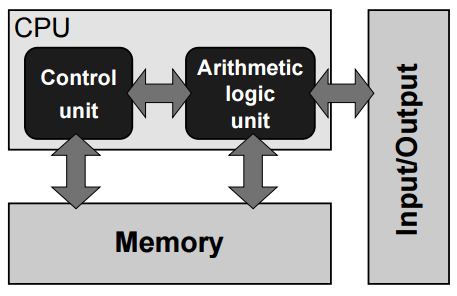
\includegraphics[width=0.6\textwidth]{stored_program_computer.png}

{\tiny From Hager and and Wellein}

\vfill

This is the basic idea for {\it all modern computers}!

\end{frame}


%------------------------------------------------------------------------------%
\begin{frame}{Stored-Program Computer -- More Realistic}

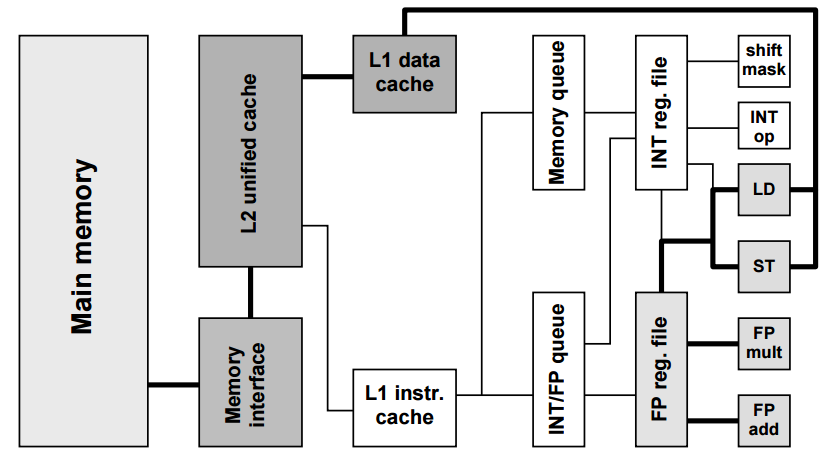
\includegraphics[width=0.8\textwidth]{cache_based_microprocessor.png}

{\tiny From Hager and and Wellein}
\vfill

{\bf Bold} lines are potential bottlenecks.

\end{frame}


%------------------------------------------------------------------------------%
\begin{frame}[fragile]{Stored-Program Computer -- Resources}

Basically, stored-program computers:
\begin{itemize}
 \item  execute instructions (design targets better throughput)
 \item  data transfer (bandwidth function of bus width, speed)
\end{itemize}

\begin{lstlisting}
  do i=1, N
     A(i) = A(i) + B(i)  
  enddo
\end{lstlisting}
\vfill 
Instructions:\\
Two loads (A(i) and B(i))\\
One add\\
One store\\
One increment\\
\vfill 
Work: N FLOPS
\vfill 
Data: 24 bytes per loop visit
\end{frame}

%------------------------------------------------------------------------------%
\begin{frame}{Advances in Processors}
 
 \begin{enumerate}
  \item superscalerity ($>1$ instruction/cycle; ``instruction level parallelism'')
  \item pipelining (decompose instruction into simple steps; each 1 cycle but on different units)
  \item out-of-order executation (e.g., organizes pipelines)
  \item ``big'' caches 
  \item RISC vs CISC 
 \end{enumerate}
 
\end{frame}

%------------------------------------------------------------------------------%
\begin{frame}{Pipelining}

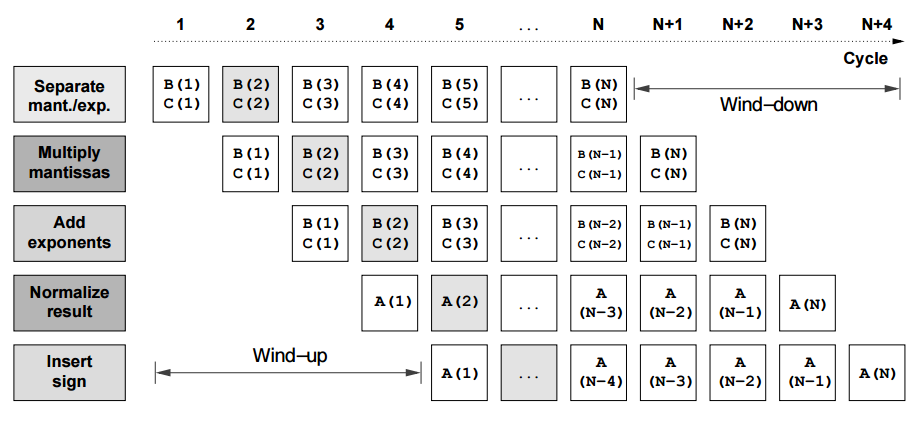
\includegraphics[width=0.8\textwidth]{fp_multiplication_pipeline.png}

{\tiny From Hager and and Wellein}
\vfill

Multiplication actually requires 5 cycles to complete!
(Division, much more...)

\end{frame}


%\section{Elements of Single-Core Optimization}


%------------------------------------------------------------------------------%
\begin{frame}{Single-Core Performance}

$P_{\text{peak}} = n_{\text{super}}  \times n_{\text{FMA}} \times n_{\text{SIMD}} \times f$

\vfill 

What are FMA and SIMD?

\end{frame}



%\section{Beyond Single-Core: Parallel Computing}


%------------------------------------------------------------------------------%
\begin{frame}{Flynn's Taxonomy}

\begin{enumerate}
 \item SISD (single instruction stream single data stream)
 \item SIMD (single instruction stream, multiple data streams)
 \item MISD (multiple instruction streams, single data stream)
 \item MIMD (multiple instruction streams, multiple data streams)
\end{enumerate}


\end{frame}



\end{document}
